


In the standard analysis, precautionary saving is modelled as the outcome of a consumer's optimizing choice of
how to allocate existing resources between the present and the future.  
The standard analysis originates in a two-period model by \cite{LelandPrecaution}, and extended to the multiperiod case
by \cite{SibleyPIH} and \cite{MillerPIH}.
Additional interest in precautionary saving was stimulated by numerical solution
of a benchmark model by \cite{zeldesStochastic} and the connection made in \cite{barskymankiwzeldes:aer} between precautionary saving and
the effects of government debt.  %The following sentence was edited
(We assume time-invariant preferences in order to sidestep the the important issues
of time consistency recently explored by \cite{laibson:goldeneggs} and others.
That literature opens up a rich and interesting field of further behavioral possibilities
beyond the basic logic outlined here.)

To clarify the theoretical issues, we break down the consumer's
problem into two steps: The transition between periods, and the choice
within the period.  A consumer who ends period $t$ with assets
${a}_{t}$ receives capital income in period $t+1$ of ${a}_{t} r$.  The
consumer's immediate resources (`cash on hand') in period $t+1$ consist of such
capital income, plus the assets that generated it, plus labor income
${y}_{t+1}$:
\begin{eqnarray}
  \label{eq:mtp1}
  {m}_{t+1} & = & {a}_{t}r+{a}_{t}+{y}_{t+1}
\\ & = & \underbrace{(1+r)}_{\equiv R}{a}_{t}+{y}_{t+1}
.
\end{eqnarray}
The simplest interpretation of ${m}$ is as the contents of the
consumer's bank account immediately after receipt of the paycheck and
interest income ('cash-on-hand'). $R$ is the real interest {\em factor}, as distinct
from the real interest {\em rate}, lower case $r$.  ${a}_{t}$ reflects
the consumer's accumulated assets at the end of period $t$, after the
spending decision for period $t$ has been made.  The transition from
the beginning to the end of period $t$ reflects the fact that spending
is paid for by drawing down ${m}$:
\begin{eqnarray}
  {a}_{t} & = & {m}_{t}-{c}_{t}.
\end{eqnarray}

To decide how to behave optimally in period $t$, the consumer must be able to judge
the value of arriving in period $t+1$ in any possible circumstance.
This information is captured by the value function
${v}_{t+1}({m}_{t+1})$.  Here, we simply assume the existence of some
well-behaved ${v}_{t+1}$; below we show how to construct ${v}_{t+1}.$

Standard practice assumes that consumers in period $t$ weight future
value by the factor $\beta$; if $\beta=1$ the consumer today cares
equally about current and future pleasure, while if $\beta<1$ the
consumer prefers present to future pleasure.  Given $\beta$, and
assuming that the consumer's period-$t$ beliefs about future
distribution of income are captured by the expectations operator
$\mathbf{E}_{t}$, we can define the value of ending period $t$ with accumulated
assets ${a}_{t}$ as
\begin{eqnarray}
  \omega_{t}({a}_{t}) & = & \beta \mathbf{E}_{t}[{v}_{t+1}(R {a}_{t}+\tilde{y}_{t+1})],
\end{eqnarray}
where the $\sim$ over the $y$ indicates that period-$(t+1)$ income
is uncertain from the perspective of period $t$.  Think of $\omega_{t}(a)$ as
the end-of-period value function.

The consumer's goal is to optimally allocate beginning-of-period resources
between current consumption and end-of-period assets; the value function
for period $t$ is defined as the function which yields the value associated
with the optimal choice:
\begin{eqnarray}
  v_{t}(m_{t}) & = & \max_{{c}_{t}} \left\{u({c}_{t}) + \omega_{t}({m}_{t}-{c}_{t})\right\}.
\end{eqnarray}
By definition the optimal choice will be a level of ${c}_{t}$ such that the consumer does not wish to change
his spending. Under standard assumptions this implies that the marginal utility of consumption must be equal to the
marginal value of assets:
\begin{eqnarray}
  u^{\prime}(\overbrace{{m}_{t}-{a}_{t}}^{{c}_{t}}) & = & \omega_{t}^{\prime}({a}_{t}) \label{eq:FOC}
,
\end{eqnarray}
since if this were not true the consumer would be able to improve
his well-being (value) by reallocating some resources either from consumption
into $a$ or from $a$ into $c$.

\begin{figure}
\caption{Marginal Utility of Assets and of Consumption} \label{fig:EquateMargUtils}
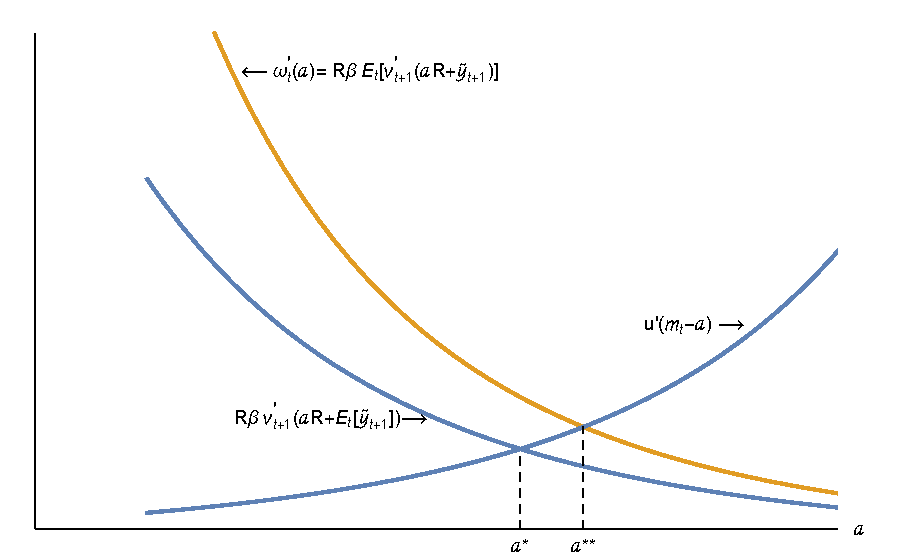
\includegraphics[width=5.5in]{./Figures/EquateMargUtils}
\end{figure}

Figure~\ref{fig:EquateMargUtils} depicts the consumer's problem
graphically.  For given initial ${m}_{t}$, the consumer's goal is to
find the value of $a$ such that \eqref{eq:FOC} holds.  The left hand
side of \eqref{eq:FOC} is the upward-sloping locus.  As for the two
downward-sloping loci, the lower one reflects expected marginal value
if the consumer is perfectly certain to receive the mean level of
income $\mathbf{E}_{t}[\tilde{y}_{t+1}]$, while the higher downward-sloping
function corresponds to the case where income is uncertain.

When the risk is added, the optimal choice for end-of-period assets
moves from ${a}^{*}$ to ${a}^{**}$. Since $c_{t} = m_{t}-a_{t}$, the
increase in $a$ in response to risk corresponds to a reduction in
consumption. This reduction in consumption is the precautionary saving
induced by the risk.

For a given ${v}_{t+1}({m}_{t+1})$, the exercise captured in the
diagram can be conducted for every possible value of $m_{t}$,
implicitly defining a consumption function $c_{t}(m_{t})$.

\cite{kimball:smallandlarge} shows that the index of absolute prudence
$\frac{-{v}^{\prime\prime\prime}_{t+1}(m_{t+1})}{{v}^{\prime\prime}_{t+1}(m_{t+1})}$
and the index of relative prudence
$\frac{-{v}^{\prime\prime\prime}_{t+1}(m_{t+1})
  m_{t+1}}{{v}^{\prime\prime}_{t+1}(m_{t+1})}$ are good measures of
how much a risk of given size will shift the marginal value of assets
curve $\omega_{t}^{\prime}(a)$ to the right.  For a constant relative
risk aversion value function, relative prudence is equal to relative
risk aversion plus one.  \cite{KimballWeil:Poss} look at the strength
of the precautionary saving motive when
Kreps-Porteus~(\citeyear{KrepsPorteus:Prefs}) preferences are used to
break the usual equation $\varsigma = 1/\rho$ where $\varsigma$ is the
elasticity of intertemporal substitution and $\rho$ is relative risk
aversion.  In this more general case, the counterpart to relative
prudence ${\cal P}$ is given by ${\cal P} = (1 + \varsigma
\varepsilon) \rho$, where $\varepsilon$ is the elasticity with which
absolute risk aversion declines and absolute risk tolerance increases.

Note that, given the basic properties $\varsigma>0$ and $\rho > 0$, a
positive wealth elasticity of risk tolerance implies that ${\cal P} >
\rho$.  This is a special case of a much more general result first
hinted at by \cite{DrezeModigliani}.  Even for very exotic objective
functions, the precautionary saving motive will always be stronger
than risk aversion whenever ownership of more $a_{t}$ due to a small
forced reduction in consumption were to lead an optimizing investor to
bear more risk (a property that Dr\`eze and Modigliani (1972) call
``endogenously decreasing absolute risk aversion''). This general
result holds because if ownership of extra $a_{t}$ due to a small
forced reduction in consumption would lead an optimizing investor to
bear risks she was previously indifferent to, then reduced consumption
must be complementary with bearing near-indifferent risks. The
symmetry of complementarity then implies that, given a free choice of
consumption levels, taking on an additional near-indifferent risk will
lead an optimizing consumer to reduce consumption. For example,
consider an agent with additive habit formation (as distinct from
multiplicative habits, cf. \cite{carroll:solvinghabits}), for whom
reduced consumption not only increases assets but reduces the size of
the consumption habit, and so unambiguously leads to more willingness
to bear risks.  Such an agent will want to reduce consumption if
induced to take on an additional risk by a compensation that makes her
indifferent to the risk.  The size of the compensation is determined
by risk aversion.  Yet the compensation for the agent's risk aversion
is not enough to cancel out the precautionary saving effect of the
risk.


\ifthenelse{\boolean{StandAlone}}{\end{document}}{}
